\documentclass[10pt,a4paper]{article}
\usepackage[margin=0.62in]{geometry}
\usepackage[T1]{fontenc}
\usepackage[utf8]{inputenc}
\usepackage{lmodern}
\usepackage{amsmath,amssymb}
\usepackage{booktabs}
\usepackage{tabularx}
\usepackage{array}
\usepackage{graphicx}
\usepackage{float}
\usepackage{subcaption}
\usepackage{enumitem}
\usepackage{xcolor}
\usepackage{hyperref}
\usepackage{microtype}
\usepackage{titlesec}
\usepackage{fancyhdr}
\usepackage[most]{tcolorbox}
\usepackage{tikz}
\usetikzlibrary{positioning,arrows.meta,calc,shapes.geometric,decorations.pathreplacing}

\definecolor{brand}{HTML}{0D3B66}
\definecolor{accent}{HTML}{2A9D8F}
\definecolor{softbg}{HTML}{F4F8FB}
\definecolor{textdark}{HTML}{1E1E1E}

\hypersetup{
  colorlinks=true,
  linkcolor=brand,
  urlcolor=accent
}

\setlength{\parindent}{0pt}
\setlength{\parskip}{3pt}
\setlist[itemize]{leftmargin=1.2em,itemsep=1pt,topsep=2pt}

\titleformat{\section}{\color{brand}\large\bfseries}{\thesection.}{0.4em}{}
\titleformat{\subsection}{\color{textdark}\bfseries}{\thesubsection}{0.4em}{}
\titlespacing*{\section}{0pt}{8pt}{4pt}
\titlespacing*{\subsection}{0pt}{6pt}{3pt}

\pagestyle{fancy}
\fancyhf{}
\fancyhead[L]{\small CS671 Technical Model Report}
\fancyhead[R]{\small Pix2Pix (Brain)}
\fancyfoot[C]{\small \thepage}
\setlength{\headheight}{14pt}

\begin{document}

% -------------------- Header Block --------------------
\begin{tcolorbox}[
  enhanced,
  colback=softbg,
  colframe=brand,
  boxrule=0.9pt,
  arc=2mm,
  left=5pt,right=5pt,top=5pt,bottom=5pt
]
\centering
{\Large\bfseries\color{brand} CS671 -- Deep Learning and Its Applications}\\[2pt]
{\large\bfseries Technical Documentation Report}\\[6pt]
{\normalsize\bfseries Model: Pix2Pix (Brain)}\\[4pt]
\small
Project Group: 5 \quad Region: Brain \quad Modality: Paired (CT $\to$ MRI)
\end{tcolorbox}

\section{ARCHITECTURAL OVERVIEW}
Pix2Pix is a conditional Generative Adversarial Network (cGAN) designed for supervised image-to-image translation. In the Brain CT-MRI task, the model learns a direct mapping from source to target modality by optimizing a combination of adversarial loss and a pixel-wise reconstruction loss, leveraging the spatial alignment of the paired dataset.

\subsection{Generator Architecture (U-Net 256)}
The generator $G_{CT \to MRI}$ is implemented as a symmetric U-Net with 8 recursive levels. Each level consists of a downsampling encoder block and a corresponding upsampling decoder block, linked by concatenation skip connections to preserve high-resolution spatial context.

\begin{figure}[H]
\centering
\resizebox{\textwidth}{!}{
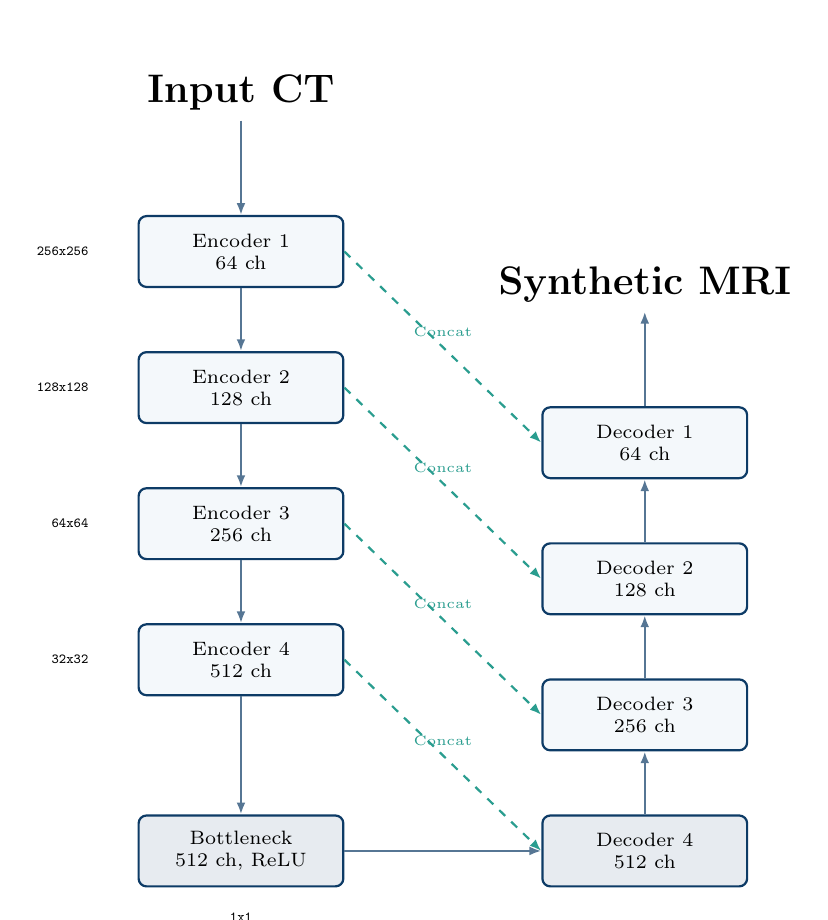
\begin{tikzpicture}[
    node distance=8mm and 2.5cm,
    block/.style={draw=brand, thick, fill=softbg, minimum width=2.6cm, minimum height=0.9cm, align=center, rounded corners=1mm, font=\scriptsize},
    ioblock/.style={draw=none, fill=none, font=\Large\bfseries, align=center},
    arr/.style={-{Latex[length=1.5mm]}, thick, draw=brand!70},
    skip/.style={-{Latex[length=1.5mm]}, thick, dashed, draw=accent}
]
    % Encoder column
    \node[block] (e1) {Encoder 1\\64 ch};
    \node[block, below=of e1] (e2) {Encoder 2\\128 ch};
    \node[block, below=of e2] (e3) {Encoder 3\\256 ch};
    \node[block, below=of e3] (e4) {Encoder 4\\512 ch};
    \node[block, below=1.5cm of e4, fill=brand!10] (bot) {Bottleneck\\512 ch, ReLU};

    % Decoder column
    \node[block, right=of bot, fill=brand!10] (d4) {Decoder 4\\512 ch};
    \node[block, above=of d4] (d3) {Decoder 3\\256 ch};
    \node[block, above=of d3] (d2) {Decoder 2\\128 ch};
    \node[block, above=of d2] (d1) {Decoder 1\\64 ch};

    % IO labels — placed ABOVE the top row, well clear of everything
    \node[ioblock, above=1.2cm of e1] (in_ct) {Input CT};
    \node[ioblock, above=1.2cm of d1] (out_mri) {Synthetic MRI};

    % Resolution labels — placed to the left, clear of IO labels
    \node[left=5mm of e1, font=\tiny\ttfamily] {256x256};
    \node[left=5mm of e2, font=\tiny\ttfamily] {128x128};
    \node[left=5mm of e3, font=\tiny\ttfamily] {64x64};
    \node[left=5mm of e4, font=\tiny\ttfamily] {32x32};
    \node[below=2mm of bot, font=\tiny\ttfamily] {1x1};

    % Connections
    \draw[arr] (in_ct) -- (e1);
    \draw[arr] (e1) -- (e2); \draw[arr] (e2) -- (e3); \draw[arr] (e3) -- (e4); \draw[arr] (e4) -- (bot);
    \draw[arr] (bot) -- (d4);
    \draw[arr] (d4) -- (d3); \draw[arr] (d3) -- (d2); \draw[arr] (d2) -- (d1);
    \draw[arr] (d1) -- (out_mri);

    % Skip connections
    \draw[skip] (e1.east) -- (d1.west) node[midway, above, font=\tiny, color=accent] {Concat};
    \draw[skip] (e2.east) -- (d2.west) node[midway, above, font=\tiny, color=accent] {Concat};
    \draw[skip] (e3.east) -- (d3.west) node[midway, above, font=\tiny, color=accent] {Concat};
    \draw[skip] (e4.east) -- (d4.west) node[midway, above, font=\tiny, color=accent] {Concat};
\end{tikzpicture}
}
\caption{Recursive U-Net Architecture: The implementation uses 8 levels of abstraction. Skip connections concatenate $n$ channels from the encoder with $n$ channels from the decoder, resulting in $2n$ input channels for the subsequent transpose convolution.}
\end{figure}

\textbf{Hierarchical Feature Extraction and Skip Pathways:} 
The generator is constructed using nested \texttt{UnetSkipConnectionBlock} modules. In the encoder, spatial dimensions are halved at each step via $4 \times 4$ convolutions with stride 2. This creates a rigorous bottleneck at $1 \times 1$ resolution (for $256 \times 256$ inputs), where global anatomical relationships are consolidated. The skip connections are critical for Brain CT-MRI translation as they allow high-resolution features like the skull's outer boundary and cortical surface edges to bypass the bottleneck, ensuring that the synthetic MRI is perfectly registered to the input CT geometry.

\textbf{Regularization and Initialization:} 
The implementation applies \texttt{Dropout(0.5)} in the three innermost decoder layers to prevent deterministic "memorization" of training pairs and improve generalization. All weights are initialized using a normal distribution with $\mu=0, \sigma=0.02$, as specified in the original Pix2Pix implementation, ensuring stable convergence of the adversarial training.

\subsection{Discriminator Architecture (Conditional PatchGAN)}
The discriminator $D_{MRI}$ is a conditional PatchGAN that takes the concatenation of the input CT and the candidate MRI as input (2-channel tensor).

\begin{figure}[H]
\centering
\resizebox{0.9\textwidth}{!}{
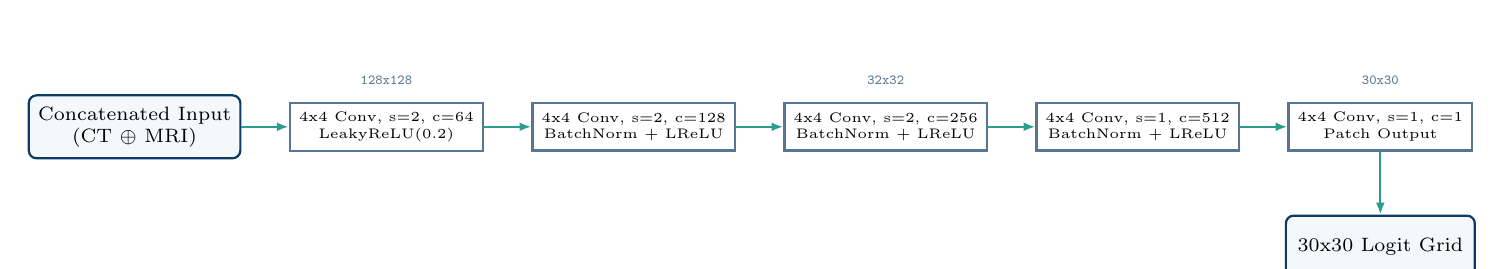
\begin{tikzpicture}[
    node distance=6mm,
    block/.style={draw=brand, thick, fill=softbg, minimum width=2.4cm, minimum height=0.8cm, align=center, rounded corners=1mm, font=\scriptsize},
    module/.style={draw=brand!70, thick, fill=white, minimum width=2.0cm, minimum height=0.6cm, align=center, font=\tiny},
    arr/.style={-{Latex[length=1.5mm]}, thick, draw=accent}
]
    \node[block] (in) {Concatenated Input\\(CT $\oplus$ MRI)};
    \node[module, right=of in] (c1) {4x4 Conv, s=2, c=64\\LeakyReLU(0.2)};
    \node[module, right=of c1] (c2) {4x4 Conv, s=2, c=128\\BatchNorm + LReLU};
    \node[module, right=of c2] (c3) {4x4 Conv, s=2, c=256\\BatchNorm + LReLU};
    \node[module, right=of c3] (c4) {4x4 Conv, s=1, c=512\\BatchNorm + LReLU};
    \node[module, right=of c4] (head) {4x4 Conv, s=1, c=1\\Patch Output};
    \node[block, below=8mm of head] (out) {30x30 Logit Grid};

    \draw[arr] (in) -- (c1); \draw[arr] (c1) -- (c2); \draw[arr] (c2) -- (c3); \draw[arr] (c3) -- (c4); \draw[arr] (c4) -- (head); \draw[arr] (head) -- (out);

    % Dimensionality
    \node[font=\tiny\ttfamily, color=brand!70, above=1mm of c1] {128x128};
    \node[font=\tiny\ttfamily, color=brand!70, above=1mm of c3] {32x32};
    \node[font=\tiny\ttfamily, color=brand!70, above=1mm of head] {30x30};
\end{tikzpicture}
}
\caption{Conditional PatchGAN: Concatenation ensures that the discriminator evaluates the joint distribution $P(CT, MRI)$, penalizing misalignments between modalities.}
\end{figure}

\textbf{Alignment-Aware Discrimination:} 
By conditioning on the CT, the discriminator learns to penalize the generator not just for poor MRI quality, but for anatomical deviations from the source CT. The output $30 \times 30$ grid classifies local patches of the image, providing a high-resolution loss signal that guides the generator to synthesize sharp edges and realistic tissue contrasts at the scale of $70 \times 70$ pixels.

\section{TRAINING DYNAMICS}
The objective function of Pix2Pix combines a conditional GAN loss with an $L_1$ reconstruction loss to enforce both perceptual realism and pixel-wise accuracy.

\begin{figure}[H]
\centering
\resizebox{0.75\textwidth}{!}{
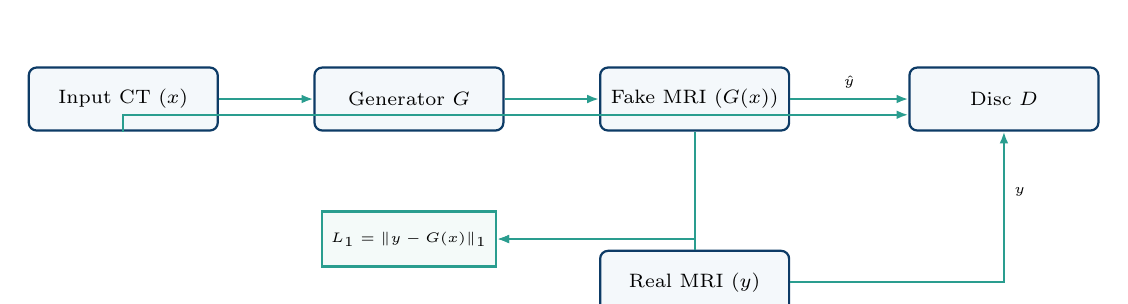
\begin{tikzpicture}[
    node distance=12mm,
    box/.style={draw=brand, thick, fill=softbg, minimum width=2.4cm, minimum height=0.8cm, align=center, rounded corners=1mm, font=\scriptsize},
    loss/.style={draw=accent, thick, fill=accent!5, minimum width=2.2cm, minimum height=0.7cm, align=center, font=\tiny\bfseries},
    arr/.style={-{Latex[length=1.5mm]}, thick, draw=accent}
]
    \node[box] (ct) {Input CT ($x$)};
    \node[box, right=of ct] (g) {Generator $G$};
    \node[box, right=of g] (fake) {Fake MRI ($G(x)$)};
    \node[box, below=1.5cm of fake] (real) {Real MRI ($y$)};
    \node[box, right=1.5cm of fake] (d) {Disc $D$};

    \draw[arr] (ct) -- (g);
    \draw[arr] (g) -- (fake);
    \draw[arr] (fake) -- (d) node[midway, above, font=\tiny] {$\hat{y}$};
    \draw[arr] (real) -| (d) node[pos=0.8, right, font=\tiny] {$y$};
    \draw[arr] (ct) |- ($(d.west) + (0,-0.2)$);
    
    \node[loss, below=1cm of g] (l1) {$L_1 = \|y - G(x)\|_1$};
    \draw[arr] (fake) |- (l1);
    \draw[arr] (real) |- (l1);
\end{tikzpicture}
}
\caption{Training workflow: Concurrent optimization of GAN and $L_1$ losses.}
\end{figure}

\textbf{Loss Objectives and Implementation Details:}
\begin{itemize}
    \item \textbf{Adversarial Loss:} Implemented using Least Squares GAN (\texttt{MSELoss}). This choice is driven by the implementation's need for bounded discriminator loss and smoother gradients, which prevents the discriminator from becoming "too strong" and halting generator progress in early epochs.
    \item \textbf{$L_1$ Reconstruction Loss:} Weighted at $\lambda = 100$, this is the primary driver for anatomical accuracy. It penalizes the absolute pixel-wise difference between the ground truth and synthetic MRI, enforcing structural fidelity.
    \item \textbf{Identity Loss (Optional):} When $\lambda_{idt} > 0$, the model is forced to learn an identity mapping if the target modality is fed as input, further regularizing the generator's behavior.
\end{itemize}

\section{INFERENCE PIPELINE}
Inference is performed as a deterministic forward pass through the trained U-Net generator.

\begin{figure}[H]
\centering
\resizebox{0.85\textwidth}{!}{
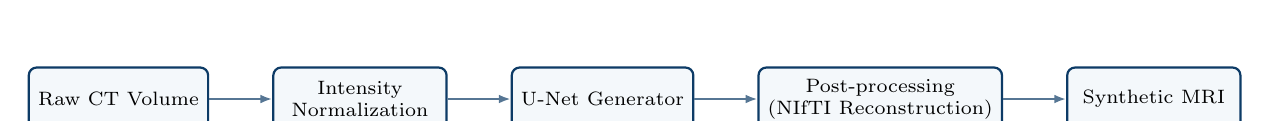
\begin{tikzpicture}[
    node distance=8mm,
    block/.style={draw=brand, thick, fill=softbg, minimum width=2.2cm, minimum height=0.8cm, align=center, rounded corners=1mm, font=\scriptsize},
    arr/.style={-{Latex[length=1.5mm]}, thick, draw=brand!70}
]
    \node[block] (in) {Raw CT Volume};
    \node[block, right=of in] (p) {Intensity\\Normalization};
    \node[block, right=of p] (g) {U-Net Generator};
    \node[block, right=of g] (r) {Post-processing\\(NIfTI Reconstruction)};
    \node[block, right=of r] (out) {Synthetic MRI};

    \draw[arr] (in) -- (p);
    \draw[arr] (p) -- (g);
    \draw[arr] (g) -- (r);
    \draw[arr] (r) -- (out);
\end{tikzpicture}
}
\caption{Inference flow: Direct translation of CT volumes to the MRI domain.}
\end{figure}

The inference system handles 3D NIfTI files by iterating through the axial stack. Each slice is normalized to the $[-1, 1]$ range used during training. The final output is rescaled to match the original MRI modality intensity distribution, facilitating direct comparison in clinical software.

\end{document}
